%%%%%%%%%%%%%%%%%%%%%%%%%%%%%%%%%%%%%%%%%%%%%%%%%%%%%%%%%%%%%%%%%%%%%%%%%%%%%%%%%%%%%%%%%%%%%%%%%%%%%%%%%%%%%%%%%%%%%
% Masters/Doctoral Thesis                                                                                           %
% LaTeX Template
% Version 1.41 (9/9/13)
%
% This template has been downloaded from:
% http://www.latextemplates.com
%
% Original authors:
% Steven Gunn 
% http://users.ecs.soton.ac.uk/srg/softwaretools/document/templates/
% and
% Sunil Patel
% http://www.sunilpatel.co.uk/thesis-template/
% 
% License:
% CC BY-NC-SA 3.0 (http://creativecommons.org/licenses/by-nc-sa/3.0/)
% 
% Note:
% Make sure to edit document variables in the Thesis.cls file
%
%%%%%%%%%%%%%%%%%%%%%%%%%%%%%%%%%%%%%%%%%%%%%%%%%%%%%%%%%%%%%%%%%%%%%%%%%%%%%%%%%%%%%%%%%%%%%%%%%%%%%%%%%%%%%%%%%%%%%%

%----------------------------------------------------------------------------------------
%	PACKAGES AND OTHER DOCUMENT CONFIGURATIONS
%----------------------------------------------------------------------------------------

\documentclass[11pt, a4paper, oneside]{Thesis} % Paper size, default font size and one-sided paper

\graphicspath{{Pictures/}} % Specifies the directory where pictures are stored
\usepackage{subfigure}
\usepackage[square, numbers, comma, sort&compress]{natbib} % Use the natbib reference package - read up on this to edit the reference style; if you want text (e.g. Smith et al., 2012) for the in-text references (instead of numbers), remove 'numbers' 
\usepackage[ruled, vlined, oldcommands, norelsize]{algorithm2e} % Use the algorithm package
\usepackage{listings}
\usepackage{xcolor}
\hypersetup{urlcolor=blue, colorlinks=true} % Colors hyperlinks in blue - change to black if annoying
\title{\ttitle} % Defines the thesis title - don't touch this

\begin{document}

\frontmatter % Use roman page numbering style (i, ii, iii, iv...) for the pre-content pages

\setstretch{1.3} % Line spacing of 1.3

% Define the page headers using the FancyHdr package and set up for one-sided printing
\fancyhead{} % Clears all page headers and footers
\rhead{\thepage} % Sets the right side header to show the page number
\lhead{} % Clears the left side page header

\pagestyle{fancy} % Finally, use the "fancy" page style to implement the FancyHdr headers

\newcommand{\HRule}{\rule{\linewidth}{0.5mm}} % New command to make the lines in the title page
\newcommand{\fortran}{\proglang{Fortran}}
% Definitions

\def \univname {New York University}
\def \ttitle {An L-BFGS-B-NS  Optimizer for Non-Smooth Functions}
\def \authornames {Wilmer Henao}
\def \supname {Michael L. Overton}
\def \degreename {Master of Science in Scientific Computing}
\def \groupname {Courant Institute of Mathematical Sciences}
\def \deptname {Department of Mathematics}
\def \subjectname {Optimization}


% PDF meta-data
\hypersetup{pdftitle={\ttitle}}
\hypersetup{pdfsubject=\subjectname}
\hypersetup{pdfauthor=\authornames}
\hypersetup{pdfkeywords=\keywordnames}

%----------------------------------------------------------------------------------------
%	TITLE PAGE
%----------------------------------------------------------------------------------------

\begin{titlepage}
\begin{center}

\textsc{\LARGE \univname}\\[1.5cm] % University name
\textsc{\Large Master's Thesis}\\[0.5cm] % Thesis type

\HRule \\[0.4cm] % Horizontal line
{\huge \bfseries \ttitle}\\[0.4cm] % Thesis title
\HRule \\[1.5cm] % Horizontal line

\begin{minipage}{0.4\textwidth}
\begin{flushleft} \large
\emph{Author:}\\
\href{http://www.johnsmith.com}{\authornames} % Author name - remove the \href bracket to remove the link
\end{flushleft}
\end{minipage}
\begin{minipage}{0.4\textwidth}
\begin{flushright} \large
\emph{Supervisor:} \\
\href{http://cs.nyu.edu/overton/}{\supname} % Supervisor name - remove the \href bracket to remove the link  
\end{flushright}
\end{minipage}\\[3cm]
 
\large \textit{A thesis submitted in fulfillment of the requirements\\ for the degree of \degreename}\\[0.3cm] % University requirement text
\textit{in the}\\[0.4cm]
\groupname\\\deptname\\[2cm] % Research group name and department name
 
{\large \today}\\[4cm] % Date
%\includegraphics{Logo} % University/department logo - uncomment to place it
 
\vfill
\end{center}

\end{titlepage}

%----------------------------------------------------------------------------------------
%	DECLARATION PAGE
%	Your institution may give you a different text to place here
%----------------------------------------------------------------------------------------

\Declaration{

\addtocontents{toc}{\vspace{1em}} % Add a gap in the Contents, for aesthetics

I, \authornames, declare that this thesis titled, '\ttitle' and the work presented in it are my own. I confirm that:

\begin{itemize} 
\item[\tiny{$\blacksquare$}] This work was done wholly or mainly while in candidature for a research degree at this University.
\item[\tiny{$\blacksquare$}] Where any part of this thesis has previously been submitted for a degree or any other qualification at this University or any other institution, this has been clearly stated.
\item[\tiny{$\blacksquare$}] Where I have consulted the published work of others, this is always clearly attributed.
\item[\tiny{$\blacksquare$}] Where I have quoted from the work of others, the source is always given. With the exception of such quotations, this thesis is entirely my own work.
\item[\tiny{$\blacksquare$}] I have acknowledged all main sources of help.
\item[\tiny{$\blacksquare$}] Where the thesis is based on work done by myself jointly with others, I have made clear exactly what was done by others and what I have contributed myself.\\
\end{itemize}
 
Signed:\\
\rule[1em]{25em}{0.5pt} % This prints a line for the signature
 
Date:\\
\rule[1em]{25em}{0.5pt} % This prints a line to write the date
}

\clearpage % Start a new page

%----------------------------------------------------------------------------------------
%	QUOTATION PAGE
%----------------------------------------------------------------------------------------

%\pagestyle{empty} % No headers or footers for the following pages

%\null\vfill % Add some space to move the quote down the page a bit

%\textit{``Thanks to my solid academic training, today I can write hundreds of words on virtually any topic without possessing a shred of information, which is how I got a good job in journalism."}

%\begin{flushright}
%Dave Barry
%\end{flushright}

%\vfill\vfill\vfill\vfill\vfill\vfill\null % Add some space at the bottom to position the quote just right

%\clearpage % Start a new page

%----------------------------------------------------------------------------------------
%	ABSTRACT PAGE
%----------------------------------------------------------------------------------------

\addtotoc{Abstract} % Add the "Abstract" page entry to the Contents

\abstract{\addtocontents{toc}{\vspace{1em}} % Add a gap in the Contents, for aesthetics

The Thesis Abstract is written here \ldots
}

\clearpage % Start a new page

%----------------------------------------------------------------------------------------
%	ACKNOWLEDGEMENTS
%----------------------------------------------------------------------------------------

\setstretch{1.3} % Reset the line-spacing to 1.3 for body text (if it has changed)

\acknowledgements{\addtocontents{toc}{\vspace{1em}} % Add a gap in the Contents, for aesthetics
I would like to thank my advisor Michael Overton for all the hours of hard work and for all the great recommendations and changes that led to this thesis.

I also would like to thank Allan Kaku and Anders Skaaja for earlier contributions to other versions of the code, and Jorge Nocedal, Ciyou Zhu, Richard Byrd and Peihuang Lu, for letting us change their original code.

Finally, I would like to thank High Performance Computing at NYU for the computing ressources and their helpful assistance.
}
\clearpage % Start a new page

%----------------------------------------------------------------------------------------
%	LIST OF CONTENTS/FIGURES/TABLES PAGES
%----------------------------------------------------------------------------------------

\pagestyle{fancy} % The page style headers have been "empty" all this time, now use the "fancy" headers as defined before to bring them back

\lhead{\emph{Contents}} % Set the left side page header to "Contents"
\tableofcontents % Write out the Table of Contents

\lhead{\emph{List of Figures}} % Set the left side page header to "List of Figures"
\listoffigures % Write out the List of Figures

\lhead{\emph{List of Tables}} % Set the left side page header to "List of Tables"
%\listoftables % Write out the List of Tables

%----------------------------------------------------------------------------------------
%	ABBREVIATIONS
%----------------------------------------------------------------------------------------

\clearpage % Start a new page

\setstretch{1.5} % Set the line spacing to 1.5, this makes the following tables easier to read

\lhead{\emph{Abbreviations}} % Set the left side page header to "Abbreviations"
%\listofsymbols{ll} % Include a list of Abbreviations (a table of two columns)
{
%\textbf{LAH} & \textbf{L}ist \textbf{A}bbreviations \textbf{H}ere \\
%\textbf{Acronym} & \textbf{W}hat (it) \textbf{S}tands \textbf{F}or \\
}


%----------------------------------------------------------------------------------------
%	DEDICATION
%----------------------------------------------------------------------------------------

\setstretch{1.3} % Return the line spacing back to 1.3

\pagestyle{empty} % Page style needs to be empty for this page

\dedicatory{Dedicated to my mother, my brother and Dr. Ian Malcolm} % Dedication text

\addtocontents{toc}{\vspace{2em}} % Add a gap in the Contents, for aesthetics

%----------------------------------------------------------------------------------------
%	THESIS CONTENT - CHAPTERS
%----------------------------------------------------------------------------------------

\mainmatter % Begin numeric (1,2,3...) page numbering

\pagestyle{fancy} % Return the page headers back to the "fancy" style

% Include the chapters of the thesis as separate files from the Chapters folder
% Uncomment the lines as you write the chapters

% Chapter 1

\chapter{Introduction} % Main chapter title

\label{Chapter1} % For referencing the chapter elsewhere, use \ref{Chapter1} 

\lhead{Chapter 1. \emph{Introduction}} % This is for the header on each page - perhaps a shortened title

%----------------------------------------------------------------------------------------
%\DeclareMathOperator*{\Min}{Min}
The goal in this thesis is to find a solution of the nonsmooth minimization problem

\begin{equation} \label{mainproblem}
  \begin{aligned}
    & \underset{x \in \mathbb{R}^n}{\text{min}}
    & & f(x) \\
    & \text{s.t.}
    & & l_i \leq x_i \leq u_i , \; \\
    & & & i = 1, \ldots, n.
  \end{aligned}
\end{equation}

where $f \colon \mathbb{R}^n \to \mathbb{R}$, $n$ is a very large but finite number. And $l_i$ and $u_i \in \mathbb{R}$

Larger problems not only mean that the problem will take a longer time to solve compared to a similar problem. But storing and calculating a Hessian matrix is prohibitively expensive. There a few techniques that have already been developed for the case when $n$ is very large and this is what we know as large scale optimization. Also, Several techniques have already been developed to handle this type of problems as long as the function $f$ is smooth. 

In this thesis $f(x)$ is a nonsmooth function.

For the particular case when $n$ is a small number, several methods that solve optimization problems of nondifferentiable functions in lower dimensions \citep{kiwiel85} have been developed. In the case of smooth functions, it is possible to use Newton iteration algorithms and achieve quadratic convergence, the problem with Newton algorithms is that they require second derivatives to be provided\footnote{the main issue with the second derivative is that it requires a total of $n \times n$ partial derivatives. Which is impractical for medium and for some small-size problems}. In the 1950's and several years after that, several quasi-newton methods were proposed where the second derivative Hessian matrix is "approximated" step by step \citep{unconstrained}. These approximations or "updates" are calculated after every iteration and the way in which this update is found defines a new method depending on the particular needs. This thesis will only be concerned with the $BFGS$. \footnote{BFGS stands for the last names of its authors Broyden, Fletcher, Goldfarb and Shanno} which can achieve super linear convergence, has proven to work in most practical purposes and posseses very nice self correcting features \citep{selfcorrecting}. In other words, it doesn't matter that one update incorrectly estimates the curvature in the objective function, $BFGS$ will always correct itself in just a few steps. This self-correcting property is very desired in the nonsmooth case, since changes in curvature could be large near the optimal point. $BFGS$ is not the right tool for large scale optimization and therefore an $L-BFGS$ adaptation is needed to solve the problem obtained on \ref{mainproblem}

A final assumption in this thesis is that the Hessian matrix is not sparse. In this case, there are other algorithms that may be more suitable \citep{Fletcher96computingsparse, sparse}, some of them have even been implemented in fortran \citep{lancelot}.

This thesis builds upon the original $L-BFGS-B$ code \citep{lbfgsbsoftware} that solves smooth problems of $f$. There were three main changes in the code. The first one is the line search conditions which required a small change in order to satisfy the different structure that a nonsmooth function requires. The second one is the line search methodology which was changed from a cubic interpolation to a bisection algorithm and last change in the thesis was the termination condition.

Nocedal's original algorithm consists of $2$ steps. In the first step most of the dimensions in the problem should be removed, making the problem a lot simpler. And in the second step there is some fine tuning to guarantee better than just linear speed of convergence.

\chapter{Original algorithm}
\label{ChapterConstraints} % For referencing the chapter elsewhere, use \ref{ChapterConstraints} 

The original algorithm \citep{mainpaper} has an accompanying software written on $FORTRAN$ \citep{lbfgsbsoftware} and this thesis builds upon that software by making sufficient changes to make it applied to the nonsmooth case.

\section{Gradient Projection}

The original algorithm was created for the case when $n$ is large and $f$ is nonsmooth. Its first step is a gradient projection similar to the one outlined in \citep{gradproj1, gradproj2} which is used to determine an active set corresponding to those variables that are bound at each step. The active set is defined at point $x^*$ is defined as:

\begin{equation}
  \begin{aligned}
    \mathcal{A}(x^*) = \{ i \in \{1 \ldots n\} |  x^*_i = l_i \vee  x^*_i = u_i\}
  \end{aligned}
\end{equation}

It seems like working on this active set is efficient in large problems and according to previous research \citep{nocedal} the gradient projection step is able to find most of the active set variables in a single stroke. 

In fact, A line search usually changes the active set by one variable at a time during the line search step \footnote{the line search is cut short immediately after the first bound is hit, so only one active constraint will change at every step. Unless the line search hits several constraints at the same time by coincidence, which is very unlikely}. So, if $1$ million constraints are active at a nondegenerate solution, at least $1$ million iterations will be needed just to get to that point.  Gradient projection gets rid of that problem, diminishing the number of iterations, and at the same reducing the number of variables for the next step.

Gradient projection works on the approximation model:

\begin{equation} \label{themodel}
  \begin{aligned}
    m_k(x) = f(x_k) + \nabla f(x_k)^T ( x - x_k) + \frac{(x - x_k)^T B_k (x - x_k) }{2}
  \end{aligned}
\end{equation}

Where $B_k$ will be a $L-BFGS-B$ approximation to the Hessian $\nabla^2 f$

In this first stage the algorithm starts on the current point $x_k$ searching on the direction of $-\nabla f(x_k)$. Whenever this search direction encounters one of the constraints, the search direction turns on the boundaries in order to remain feasible. The path is nothing but the feasible piecewise projection of the steepest descent search direction on the contraint "box" determined by the values $\overrightarrow{l}$ and $\overrightarrow{u}$. At the end of this stage, the value of $x$ that minimizes $m_k(x)$ on this piecewise gradient projection path is known as the "Cauchy point" $x^c$.

\subsection{Subspace Minimization}

The problem with gradient projection is that it eventually becomes steepest descent. In fact, gradient projection is exactly steepest descent if it were not for the existence of the constraints. The main problem with steepest descent is that it does not take advantage of the information of the curvature of the function which causes it to have a slow speed of convergence (linear). It is for this reason that a stage two is necessary. Define the working set as the active set defined on the cauchy point $\mathcal{A}(x^c)$. In order to do this, solve the quadratic subproblem in which all values of the working set $\mathcal{A}(x^c)$ are fixed at the values corresponding to $x^c$


The final step on this alrorithm is the subspace minimization. Once the gradient direction step has been taken, several dimensions in the problem will have been removed. Here, the algorithm takes advantage of this situation and solves the quadratic model \ref{themodel} restricted to the simple constraints. In order to do this, a new search direction is proposed. And the step length is such that it stays within the bounds stablished in the problem.

The idea at a higher level is to solve the constrained problem, but only on those dimensions that are free (not at bound). In the notation set forth in the previous algorithm. $\mathcal{F}$ represents the set of indices corresponding to the $t$ free variables. $Z_k$ is the matrix formed by the $t$ unit vector columns that span the dimensions of the free variables and $A_k$ is the corresponding matrix that represents the active constraint gradient (also unit vectors). The dimension of $Z_k$ would be $n \times t$ and the dimension of $A_k$ $n \times (n - t)$.

The starting point for this new problem will be the previously found cauchy point $x^c$, and the algorithm only moves in a direction that lives in the space generated by the columns of $Z_k$. In other words, if $\hat{d}$ is the $t$-dimensional search direction,  

\begin{equation} \label{dirconst}
  \begin{aligned}
    x = x^c + Z_k \hat{d}
  \end{aligned}
\end{equation}

Under this equation and replacing in \ref{themodel}, it's obtained

\begin{equation} \label{themodelrestr}
  \begin{aligned}
    m_k(x) = \hat{d}^T\hat{r}^c + \frac{1}{2} \hat{d}^T \hat{B}_k \hat{d} + \gamma
  \end{aligned}
\end{equation}

where $\gamma$ is a constant and $\hat{B}_k = Z_k^T B_k Z_k$, or the Hessian restricted to the "free" dimensions in the problem. $\hat{r}^c = Z^T_k (g_k + B_k(x^c - x_k))$ is the corrected gradient restricted to the same "free" dimensions. Which restates the problem as

\begin{equation} \label{subproblem}
  \begin{aligned}
    & \underset{\hat{d} \in \mathbb{R}^t}{\text{min}} 
    & & \hat{m}_k(\hat{d}) = \hat{d}^T\hat{r}^c + \frac{1}{2} \hat{d}^T\hat{B}_k\hat{d} + \gamma \\
    & \text{s.t.}
    & & l_i - x_i^c \leq \hat{d}_i \leq u_i - x_i^c , \; \\
    & & & i \in \mathcal{F}
  \end{aligned}
\end{equation}

And the solution is simply $\hat{d}^u = -\hat{B}_k^{-1}\hat{r}^c$\footnote{Notice that this implies the inversion of $\hat{B}_k$. However there is a numerical trick explained in \citep{nocedal}, that makes this operation trivial, since $\hat{B}_k$ is a small-rank correction of a diagonal matrix and its inverse can be computed by the Sherman-Morrison-Woodbury formula}. Now the step length should be $\hat{d}^* = \alpha^* \hat{d}^u$ where $\alpha^*$ is chosen so that the new point $\bar{x}_i$ stays within the constraints originally imposed.

\chapter{Modifications to the original algorithm}

\section{Convex Hull and termination conditions}

The most important requirement of a practical algorithm is that it ends in a finite time. For the case of smooth functions, the formal way to do this is to check whether the gradient has dimension zero $0$ wherever the constraints are not at bound. In the case of nonsmooth functions however, this is not necessarily true and the function at the minimum, may have a kink. In this kink the gradient may not vanish. Furthermore, if there is a sequence of points that approaches the optimum $x$ from the right, the gradients corresponding to this sequence of points might be completely different from the gradients associated to a sequence gradients associated to a sequence of points that approaches the optimum from the left. In other cases, the optimum might be located right at one of the boundaries, In this case the gradient does not necessarily vanish.

Given this set of conditions, there is the need for a special set of rules to establish the finalization of each optimization.

Since BFGS approximations typically converge to Clarke-Stationary points. The right methodology is to calculate the subgradient. One particular methodology that guarantees an end to the algorithm is suggested in \citep{overtonlewis}. In order to make sure that the gradient zero $\vec{0}$ is part of the subgradient calculated over a neighbourhood of the optimum.
The algorithm keeps a record of the latest gradient vectors in a small neighbourhood of the point that we suspect is the optimum, This collection is called $G_k$ in \citep{overtonlewis}, This collection of gradients spans an associated convex hull of gradients. If this convex hull contains at least one vector of dimension smaller than a tiny number $\tau_k$, the algorithm ends.

Of course the best way to find a vector with such properties is to find the vector with the minimal norm that resides in the convex hull generated by $G_k$

\subsubsection{minimization of the quadratic program}

This solution is guarantees to end up at a local optimum. However, one subalgorithm needs to be solved. This algorithm is a practical primal-dual algorithm. In this case in particular the best solution is to implement a variation of Mehrotra's Predictor-Corrector algorithm applied to quadratic programming. The primal dual method requires the solution of a system in order to calculate the search direction. The most expensive part of this solution is the calculation of the cholesky decomposition. Mehrotra's algorithm uses the same cholesky decomposition to calculate both directions. the predictor, and the corrector.

Currently there is not a theoretical calculation of the complexity of this algorithm but it is very used in practice. The implementation here is exactly the one on \citep{Nocedal}. It was implemented in fortran as part of the optimizer.

\section{cubic interpolation replaced with line search}

The original software by Nocedal\citep{Nocedal}, included a cubic line search. The idea of a cubic interpolation line search is to take advantage of the smooth properties of functions and take advantage of the curvature properties. It is debatable to see which one works better whether a simple line search or a cubic interpolation. However, In the case of nonsmooth functions, this line search does not serve our purpose and therefore a more typical line search that implements a bisection was used.

In general, a step length is selected. If this step length does not satisfy the sufficient decrease and curvature conditions, then a step length of half or double the size is selected. the algorithm is guaranteed to converge under a careful selection of the parameters, however, in case this does not happen, the software will stop with a warning. 

\section{the functions to be tested}

In order to make some tests, a few functions will be evaluated. The most important function to test this non-smooth optimizer is a modified version of rosenbrock's:

\begin{equation}
    f(x) = (x_1 - 1)^2 + \sum_{i = 2}^n |x_i - x_{i - 1}^2|^p
\end{equation}

Where the value of $p$ changes the behaviour of the optimizer. This function can be proven to be lipschitz continuous whenever $p > 1$ if restricted to the domain defined by 

\begin{equation}
  \begin{aligned}
    x_i = 
    \begin{cases}
      [-100, 100] & \text{if } i \in \text{ even numbers} \\
      [10, 100] & \text{if } i \in \text{ odd numbers}
    \end{cases}
  \end{aligned}
\end{equation}

and in fact, whenever the function is restricted to a finite domain. Because whenever $p > 1$ we have that the function $f(z) = |z|^p$ is zero $0$ around zero because the derivative $p |z| ^{p-1}$ is zero whenever $z$ tends to zero from the right. (from the left also because it is an even function). However the second derivative will not be as nice.

For the case when $p \leq 1$ we have that the second derivative tends to infinity. $\displaystyle \lim_{x \to 0^+} {f' = \infty}$. Which is already well known given the "heavyside" look of $f(z) = |z|$.

The convergence of the algorithm smoothly descends to the objective 
\centering
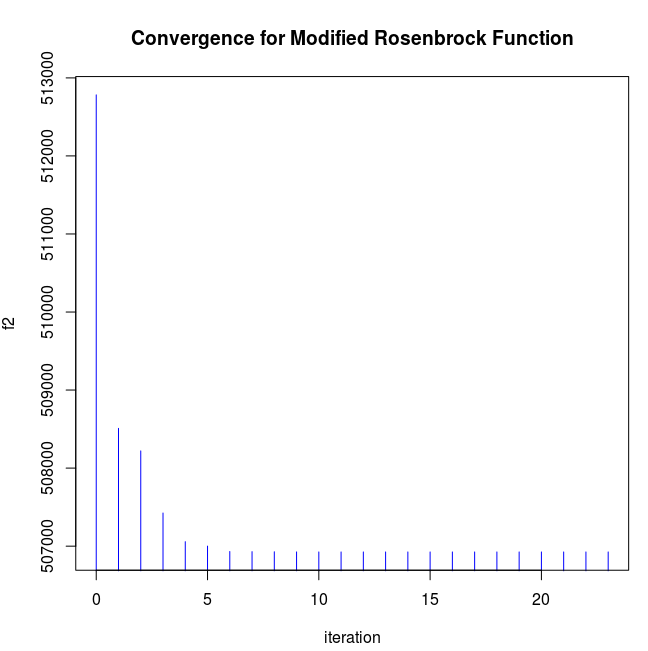
\includegraphics[scale=0.3]{Figures/convergence.png}

The converge is adversely affected by the selection of $p$ as one would expect. Values of $p$ descending to $1$ make the function less "smooth" and have the adverse effect of making the convergence much more difficult. In this exercise it is noticeable how slow the convergence becomes for a few specific values of $p$. In particular for $1.0001$

\centering
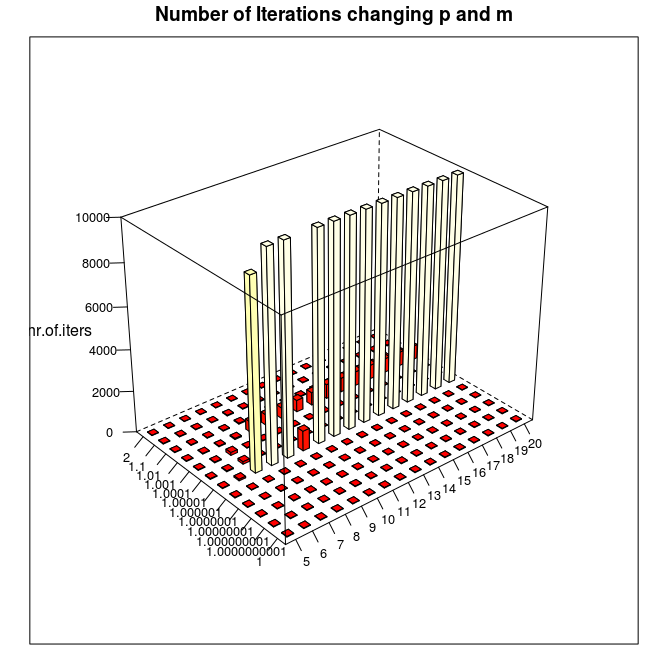
\includegraphics[scale=0.3]{Figures/hist3dmpniter.png}

\section{Weak wolfe conditions}

Probably the most important change made to the original code was the change in the curvature condition. Originally there are two Wolfe conditions, one of them is the Armijo condition, also known as the sufficient decrease conditions.

\begin{equation}
  \begin{aligned}
    f(x_k + \alpha_kp_k) \leq f(x_k) + c_1 \alpha _k p_k^T\nabla f(x_k)
  \end{aligned}
\end{equation}

and the other one is the curvature condition, of which the most popular version is the strong wolfe curvature condition:

\begin{equation}
  \begin{aligned}
    |p_k^T \nabla f(x_k + \alpha _k p_k)| \leq |p_k^T \nabla f(x_k)|
  \end{aligned}
\end{equation}

The strong wolfe is a more natural way to see and achieve convergence, but the problem is that it does not work well for the nonsmooth case. This is because near the minimal points, there maybe abrupt changes in curvature, in these cases there is no other option but to relax the curvature condition as long as the sufficient decrease condition is satisfied. The suggested new decrease condition is this.

\begin{equation}
  \begin{aligned}
    p_k^T \nabla f(x_k + \alpha _k p_k) \geq p_k^T \nabla f(x_k)
  \end{aligned}
\end{equation}

It is noticeable that with this new condition the algorithm does not crash, as opposed to when the hard wolfe condition is used.

%\input{Chapters/Chapter2} 
%\input{Chapters/Chapter3}
%\chapter{Experimental Results}
\lhead{Chapter 4. \emph{Experimental Results}}

The \texttt{L-BFGS-B} implementation was tested on the high performance cluster machines at NYU. In order to run these tests it was necessary to create a series of PBS files\footnote{PBS stands for Portable Batch System. This is software that performs job scheduling. It is used by High Performance Computing at NYU (and many other High Performance Computing Centers) to allocate computational tasks. In order to run jobs at the high performance clusters, a series of PBS batch files need to be created.} using a PBS generator script. This script generator created PBS files which in turn run bash shell scripts\footnote{Bash is a command processor. Each Bash script that was created includes a series of computer commands, namely, execution of the original \texttt{L-BFGS-B} software and the new code \texttt{L-BFGS-B-NS}.}. Several of these shell scripts are available at the repository \citep{lbfgsbNS}. The main reason to run scripts this way is because it achieves parallelism, and because the system sends confirmation e-mails and statistics about the different stages of the processes giving a lot of control to the practitioner.

\section{Exit Messages}

The original \texttt{L-BFGS-B} optimizer displays different messages depending on the condition that triggered the exit. The following is a list of some of the most common exit messages in the original \texttt{L-BFGS-B} optimizer along with an explanation of how we generalized them in \texttt{L-BFGS-B-NS}.

\begin{itemize}

\item ``ABNORMAL\_TERMINATION\_IN\_LNSRCH'' This message means that there was a problem with the line search and the program's exit was premature. In \texttt{L-BFGS-B}, it typically occurs for non-smooth functions where the line search breaks down. In \texttt{L-BFGS-B-NS}, it typically occurs when the limit on the number of bisections in the line search ($30$) is exceeded.

\item ``CONVERGENCE: NORM\_OF\_PROJECTED\_GRADIENT\_LT\_PGTOL": Means that convergence was achieved because the norm of the projected gradient is small enough. We made just one change to the original \texttt{L-BFGS-B} code: in order to have results that are comparable with the results obtained with the new code, we terminated when the $2$-norm of the projected gradient was less than the tolerance $\tau =10^{-6}$, instead of the $\infty$-norm. Notice that this convergence message does not apply to \texttt{L-BFGS-B-NS} because of particular requirements for non-smooth functions involving the convex hull of projected gradients as explained in section \ref{terminator}. Instead it is replaced by:

\item ``CONVERGENCE: ZERO\_GRAD\_IN\_CONV\_HULL" This means that the termination condition discussed in section \ref{terminator} was satisfied\footnote{This does not mean that the resulting vector is exactly equal to zero $0$, but it is small enough to satisfy the termination condition.}. We set $\tau_d = 10^{-6}$ and $\tau_x = 10^{-3}$

\item ``CONVERGENCE: REL\_REDUCTION\_OF\_F\_LT\_FACTR*EPSMCH": This convergence condition is achieved whenever the relative reduction of the value of function $f$ is smaller than a predefined factor times the machine precision $\epsilon$. This exit message does not apply to our tests. It was disabled by setting the factor ``FACTR'' to zero, both in our runs of \texttt{L-BFGS-B-NS} and our tests using the original code \texttt{L-BFGS-B}.

\end{itemize}

The limit on the number of iterations was set to $10000$.

\section{Modified Rosenbrock Function} \label{ros}

Consider a modified version of the Rosenbrock function problem \citep{rosenbrock}:

\begin{equation} \label{modifiedrosenbrock}
    f(x) = (x_1 - 1)^2 + \sum_{i = 2}^n |x_i - x_{i - 1}^2|^p
\end{equation}

We can study the properties of function $f$ based on the properties of the function $\phi(t_i)$, where $\phi(t_i) = |t_i|^p$ and $t_i = x_i - x_{i - 1}^2$. The properties of the function depend on the value of the $p$ parameter\footnote{The original Rosenbrock function had a value of $p = 2$ and the second term was multiplied by $100$.}. This function can be proven to be locally Lipschitz continuous whenever $p \geq 1$. However, its second derivative blows up at zero whenever $p < 2$. Note that although $\phi(t_i)$ is convex for $p \geq 1$, $f$ is not convex.

The properties of $\phi(t_i)$ can be separated into different cases. Whenever $p > 1$ the derivative can be represented as:
\begin{equation}\label{firstderiv}
  \frac{d}{dt} \phi(t) = \pm p |t|^{p-1}
\end{equation}
and therefore, the limit of the derivative exists and is equal to zero near $t = 0$: \[ \lim_{t \to 0} \frac{d}{dt}\phi(t) = 0 \] From this we conclude that $f$ has a smooth first derivative for $p > 1$.

However, if $p = 1$, $\phi(t) = |t|$, and the absolute value function is not differentiable at $t = 0$. Note that in this case, $\phi(t)$ is Lipschitz continuous at $t = 0$.

The second derivative provides a bit more of information.

\begin{equation}\label{secondderiv}
  \frac{d^2}{dt^2} \phi(t) = \pm p(p-1) |t|^{p-2}
\end{equation}

If $p \geq 2$ the function is twice continuously differentiable. However if $p < 2$, the second derivative becomes $\frac{p(p-1)}{|t|^{q}}$, where $q = 2 - p > 0$, and this second derivative blows up as $|t| \to 0$. The special case $p = 1$ has second derivative equal to zero since $p(p-1) = 0$ except at $t = 0$ where it is undefined. For $p < 1$, $\phi$ is not Lipschitz continuous at $t = 0$

Having explained the characteristics of the function, the next thing that needs to be defined is the region to be tested. We chose the region to be defined by the ``box'' with boundaries

\begin{equation}
  \begin{aligned}
    x_i = 
    \begin{cases}
      [-100, 100] & \text{if } i \in \text{ even numbers} \\
      [10, 100] & \text{if } i \in \text{ odd numbers}
    \end{cases}
  \end{aligned}
\end{equation}

The initial point was chosen to be the midpoint of the box, plus a different small perturbation for each dimension, chosen so that the line search does not reach the boundary of several dimensions in one step:

\begin{equation}
  \begin{aligned}
    x_i = \frac{u_i + l_i}{2} - \left(1 - 2^{1 - i}\right)
  \end{aligned}
\end{equation}

It is important to note that this choice of initial point makes the problem more difficult to solve. The problem is easier if the midpoint is chosen.

The problem is twice continuously differentiable for values of $p \geq 2$, but as the values of $p$ approach $1$, we expect the original \texttt{L-BFGS-B} optimizer to start to have difficulties. We tested both the original \texttt{L-BFGS-B} optimizer and the new code \texttt{L-BFGS-B-NS} on the modified Rosenbrock function with $p$ varying between $2$ and $0.9$ and $n$ varying between $100$ and $10000$, with the variable memory parameter $m$ set to $5$, $10$ and $20$.

For the value $p = 2$, the original \texttt{L-BFGS-B} yields good results as seen in Table \ref{pequal2}.

\begin{center}
  \begin{table}
    \begin{center}
      \scriptsize
      \begin{tabular}{|l|l|l|l|l|l|l|l|l|l|l|}
        \hline
      p &  n  &  m  & \multicolumn{4}{|c|}{\texttt{L-BFGS-B} results} & \multicolumn{4}{|c|}{\texttt{L-BFGS-B-NS} results} \\ \hline
        & &  & iters. & \#fg & f & NPG & iters. & \#fg & f & NSVCHPG \\ \hline
      2 &  100 & 5 & 29 & 131 & 452116.014385974 & 2.92E-06 & 34 & 67 & 452116.014385974 & 1.46E-08\\
      2 &  100 & 10  & 25 & 67 & 452116.014385974 & 7.37E-05 & 32 & 45 & 452116.014385974 & 2.29E-07\\
      2 &  100 & 20  & 25 & 28 & 452116.014385974 & 8.97E-07 & 29 & 47 & 452116.014385974 & 1.20E-04\\
      2 &  200 & 5 & 32 & 74 & 913376.515331672 & 1.97E-07 & 34 & 62 & 913376.515331677 & 8.44E-07\\
      2 &  200 & 10  & 27 & 32 & 913376.515331672 & 5.26E-07 & 32 & 43 & 913376.515331672 & 1.04E-07\\
      2 &  200 & 20  & 26 & 29 & 913376.515331672 & 5.80E-07 & 33 & 58 & 913376.515331677 & 3.98E-08\\
      2 &  1000 & 5  & 26 & 68 & 4603460.52289722 & 2.61E-04 & 37 & 80 & 4603460.52289732 & 9.85E-07\\
      2 &  1000 & 10  & 26 & 71 & 4603460.52289722 & 5.93E-04 & 33 & 45 & 4603460.52289733 & 5.89E-07\\
      2 &  1000 & 20  & 30 & 95 & 4603460.52289722 & 1.18E-05 & 33 & 59 & 4603460.52289732 & 9.02E-07\\
      2 & 5000 & 5 & 27 & 122 & 23053880.5607232 & 4.44E-03 & 23 & 41 & 23053880.5607253 & 2.19E-07\\
      2 & 5000 & 10 & 25 & 28 & 23053880.5607256 & 8.96E-07 & 32 & 40 & 23053880.5607253 & 8.40-07\\
      2 & 5000 & 20 & 26 & 80 & 23053880.560724 & 3.75E-03 & 17 & 43 & 23053880.5607232 & 1.08E-07\\
      2 & 10000 & 5 & 26 & 68 & 46116905.6080045 & 2.80E-06 & 12 & 232 & 46116905.6079994 & 5.41E-06\\
      2 & 10000 & 10 & 25 & 67 & 46116905.6080057 & 7.70E-03 & 18 & 297 & 46116905.6080044 & 3.66E-05\\
      2 & 10000 & 20 & 28 & 73 & 46116905.608006 & 5.18E-06 & 18 & 297 & 46116905.6080044 & 3.66E-05\\
      \hline
      \end{tabular}
      \caption[Modified Rosenbrock with $p = 2$]{Satisfactory results for the original algorithm \texttt{L-BFGS-B}  and for \texttt{L-BFGS-B-NS} applied to the Modified Rosenbrock function with $p = 2$. NPG: Norm of projected Gradient with tolerance $10^{-6}$. 
NSVCHPG: Norm of Smallest Vector in Convex Hull of Projected Gradients with $\tau_d = 10^{-6}, \tau_x = 10^{-3}$}
      \label{pequal2}
    \end{center}
  \end{table}
\end{center}

\subsection{Performance of \texttt{L-BFGS-B} and \texttt{L-BFGS-B} on the Modified Rosenbrock Function}

On the tables, iters shows the number of iterations, $\#fg$ shows the number of function and gradient evaluations taken, and $f$ shows the final computed function value that was achieved by the optimization. \emph{NPG} shows the norm of the projected gradient. The termination tolerance for the euclidean norm of the projected gradients was $10^{-6}$. In most cases this test was satisfied.

In the case of \texttt{L-BFGS-B-NS} \emph{NSVCHPG} shows the norm of the smallest vector in the convex hull of projected gradients. We can see that since this function is smooth when $p = 2$, \texttt{L-BFGS-B} has no problems solving the test and that \texttt{L-BFGS-B-NS} reaches exactly the same values, although because of the line search changes, the number of iterations and function and gradient evaluations usually increases.

\begin{table}
  \scriptsize
  \begin{center}
    \begin{tabular}{|l|l|l|l|l|l|l|l|l|l|l|}
      \hline
      p  &  n  &  m  & \multicolumn{4}{|c|}{\texttt{L-BFGS-B} results} & \multicolumn{4}{|c|}{\texttt{L-BFGS-B-NS} results} \\ \hline
      & &  & iters. & \#fg & f & NPG & iters. & \#fg & f & NSVCHPG \\ \hline
      1 & 100 & 5  & 1 & 21 & 151292.8 & 7.79E+02 & 15 & 130 & 4826.1066601788 & 1.34E-08\\
      1 & 100 & 10  & 1 & 21 & 151292.8 & 7.79E+02 & 15 & 129 & 4826.1066352341 & 1.34E-08\\
      1 & 100 & 20  & 1 & 21 & 151292.8 & 7.79E+02 & 15 & 129 & 4826.1066352341 & 1.34E-08\\
      1 & 200 & 5  & 1 & 21 & 299792.8 & 1.10E+03 & 15 & 128 & 9668.0522943829 & 1.82E-08\\
      1 & 200 & 10  & 1 & 21 & 299792.8 & 1.10E+03 & 15 & 128 & 9668.0522930362 & 1.82E-08\\
      1 & 200 & 20  & 1 & 21 & 299792.8 & 1.10E+03 & 15 & 112 & 9667.9345180734 & 1.19E-07\\
      1 & 1000 & 5  & 1 & 21 & 1487792.8 & 2.46E+03 & 23 & 193 & 48403.1390323475 & 5.72E-09\\
      1 & 1000 & 10  & 1 & 21 & 1487792.8 & 2.46E+03 & 16 & 160 & 48403.3203939957 & 2.44E-08\\
      1 & 1000 & 20  & 1 & 21 & 1487792.8 & 2.46E+03 & 16 & 160 & 48403.320394002 & 2.44E-08\\
      1 & 5000 & 5 & 1 & 21 & 7427792.8 & 5.51E+03 & 20 & 127 & 242078.712084738 & 1.26E-08\\
      1 & 5000 & 10 & 1 & 21 & 7427792.8 & 5.51E+03 & 56 & 339 & 242078.839910433 & 1.26E-08\\
      1 & 5000 & 20 & 1 & 21 & 7427792.8 & 5.51E+03 & 45 & 249 & 242078.560631846 & 7.84E-08\\
      1 & 10000 & 5 & 1 & 21 & 14852792.8 & 7.79E+03 & 18 & 148 & 484172.781463252 & 8.25E-08\\
      1 & 10000 & 10 & 1 & 21 & 14852792.8 & 7.79E+03 & 10000 & 20019 & 484269.73074638832 & 3.76E+02 \\
      1 & 10000 & 20 & 1 & 21 & 14852792.8 & 7.79E+03 & 21 & 101 & 484172.918293261 & 1.77E-08\\
      \hline
    \end{tabular}
    \caption[Modified Rosenbrock with $p = 1$]{Unsatisfactory results for the original algorithm \texttt{L-BFGS-B} applied to the Modified Rosenbrock function with $p = 1$. And converging results for \texttt{L-BFGS-B-NS}; NPG: Norm of projected Gradient with tolerance = $10^{-6}$. NSVCHPG: Norm of Smallest Vector in Convex Hull of Projected Gradients with $\tau_d = 10^{-6}, \tau_x = 10^{-3}$}
    \label{pequal1merged}
  \end{center}
\end{table}

On the other hand, the value of $p = 1$ leads to an abnormal line search termination for \texttt{L-BFGS-B} in all of the cases presented. This is to be expected as the function is non-smooth. See table \ref{pequal1merged} where the norm of the resulting projected gradient never approaches zero. In this exercise, the memory length $m$ of \texttt{L-BFGS}, does not have an impact on the final value $f$ of the optimization, but this is because all cases terminated before the $5^{th}$ iteration and therefore all different cases of $m$ end up looking exactly the same.

In fact, for all cases \texttt{L-BFGS-B} crashes in the first iteration with a value very distant from any local optimum.  \texttt{L-BFGS-B-NS} on the other hand is able to converge under most scenarios. In fact, it is possible to converge under all scenarios by tweaking the starting point of the optimization.

Several other values of $p$ were also tested. In table \ref{pmtable}, the parameter $p$ is varied and all other parameters are held constant, among others $1.1$, $1.01$, $1.001$, ... , $1.00001$, $1$. With a tolerance of $10^{-6}$ \texttt{L-BFGS-B} always fails as expected, and those values where $p$ is closer to $1$ are the most difficult for the original algorithm to handle.  Values generated via \texttt{L-BFGS-B-NS} are comparatively better whenever $p < 2$, since the function is ``less'' smooth. Most runs of \texttt{L-BFGS-B-NS} converge using the termination condition from section \ref{terminator}.

\begin{table}
  \tiny
  \begin{center}
    \begin{tabular}{|l|l|l|l|l|l|l|l|l|l|l|}
      \hline
      p & n & m  & \multicolumn{4}{|c|}{\texttt{L-BFGS-B} results} & \multicolumn{4}{|c|}{\texttt{L-BFGS-B-NS} results} \\ \hline
      &  & & iters. & \#fg & f & NPG & iters. & \#fg & f & NSVCHPG \\ \hline
      2 & 200 & 5 & 32 & 74 & 913376.515331672 & 1.97E-07 & 35 & 55 & 913376.515331676 & 3.19E-09\\
      2 & 200 & 10  & 27 & 32 & 913376.515331672 & 5.26E-07 & 20 & 41 & 913376.515331677 & 3.98E-07\\
      2 & 200 & 20 & 26 & 29 & 913376.515331672 & 5.80E-07 & 19 & 40 & 913376.515331672 & 8.03E-07\\
      1.5 & 200 & 5 &  8 & 50 & 95144.1877450699 & 9.60E+02 & 29 & 68 & 94261.6310280216 & 7.52E-07\\
      1.5 & 200 & 10 &  8 & 50 & 95095.5635531693 & 9.61E+02 & 30 & 59 & 94261.6310280212 & 9.69E-07\\
      1.5 & 200 & 20 &   8 & 50 & 95095.5635531693 & 9.61E+02 & 26 & 66 & 94261.6310280211 & 9.95E-07\\
      1.1 & 200 & 5 &  1 & 21 & 658485.96769483 & 1.10E+03 & 26 & 75 & 15226.525226329 & 4.24E-07\\
      1.1 & 200 & 10 &  1 & 21 & 658485.96769483 & 1.10E+03 & 34 & 107 & 15226.5210644821 & 1.16E-07\\
      1.1 & 200 & 20 &  1 & 21 & 658485.96769483 & 1.10E+03 & 38 & 99 & 15226.5209960549 & 1.73E-07\\
      1.01 & 200 & 5 &  1 & 21 & 324235.017102379 & 1.10E+03 & 31 & 305 & 10218.0196721806 & 3.64E+01\\
      1.01 & 200 & 10 &  1 & 21 & 324235.017102379 & 1.10E+03 & 47 & 151 & 10116.5275434197 & 7.29E-07\\
      1.01 & 200 & 20 &  1 & 21 & 324235.017102379 & 1.10E+03 & 29 & 123 & 10116.5603888173 & 2.95E-09\\
      1.001 & 200 & 5 &  1 & 21 & 302150.58179968 & 1.10E+03 & 36 & 111 & 9711.8763115237 & 5.70E-08\\
      1.001 & 200 & 10 &  1 & 21 & 302150.58179968 & 1.10E+03 & 23 & 100 & 9711.8906439951 & 2.81E-09\\
      1.001 & 200 & 20 &  1 & 21 & 302150.58179968 & 1.10E+03 & 39 & 164 & 9711.876311317 & 1.41E-07\\
      1.0001 & 200 & 5 &  1 & 21 & 300027.736327598 & 1.10E+03 & 306 & 638 & 9672.3210642275 & 5.09E-07\\
      1.0001 & 200 & 10 &  1 & 21 & 300027.736327598 & 1.10E+03 & 17 & 96 & 9672.3639815678 & 1.82E-08\\
      1.0001 & 200 & 20 &  1 & 21 & 300027.736327598 & 1.10E+03 & 19 & 96 & 9672.3922445339 & 2.80E-09\\
      1.00001 & 200 & 5 &  1 & 21 & 299816.285236336 & 1.10E+03 & 27 & 96 & 9668.3934739514 & 4.32E-07\\
      1.00001 & 200 & 10 &  1 & 21 & 299816.285236336 & 1.10E+03 & 15 & 80 & 9668.373073478 & 2.80E-09\\
      1.00001 & 200 & 20 &  1 & 21 & 299816.285236336 & 1.10E+03 & 15 & 80 & 9668.3730743134 & 2.80E-09\\
      1 & 200 & 5 & 1 &  21  & 299792.8 & 1.10E+03 & 15 & 128 & 9668.0522943829 & 1.82E-08\\
      1 & 200 & 10 & 1 &  21 & 299792.8 & 1.10E+03 & 15 & 128 & 9668.0522930362 & 1.82E-08\\
      1 & 200 & 20 & 1 &  21 & 299792.8 & 1.10E+03 & 15 & 112 & 9667.9345180734 & 1.19E-07\\
      \hline
    \end{tabular}
    \caption[Number of algorithm Iterations Changing $p$]{This is the number of algorithm iterations for different values of $p$. $n = 200$, $m = 10$ and $\tau_d = 10^{-6}, \tau_x = 10^{-3}$ and the tolerance of \texttt{L-BFGS-B} is $10^{-6}$ }
    \label{pmtable}
  \end{center}
\end{table}

Finally, some runs with a value of $p = 0.999$ on Table \ref{p0999}. As it can be seen, both algorithms fail in the sense that the termination criteria are never met, but \texttt{L-BFGS-B-NS} reaches a better feasible solution in every scenario

\begin{table}
  \tiny
  \begin{center}
    \begin{tabular}{|l|l|l|l|l|l|l|l|l|l|l|}
      \hline
      p  & n & m  & \multicolumn{4}{|c|}{\texttt{L-BFGS-B} results} & \multicolumn{4}{|c|}{\texttt{L-BFGS-B-NS} results} \\ \hline
      &  &  & iters. & \#fg & f & NPG & iters. & \#fg & f & NSVCHPG \\ \hline
      0.999 & 100 & 5 & 1 & 21 & 150123.179035242 & 7.79E+02 & 10000 & 20003 & 4900.9128213197 & 3.86E+01\\
      0.999 & 100 & 10 & 1 & 21 & 150123.179035242 & 7.79E+02 & 10000 & 19999 & 4900.9123782223 & 3.79E+01\\
      0.999 & 100 & 20 & 1 & 21 & 150123.179035242 & 7.79E+02 & 10000 & 20000 & 4900.8873111184 & 3.78E+01\\
      0.999 & 200 & 5 & 1 & 21 & 297453.671572579 & 1.10E+03 & 10000 & 29971 & 9720.7074076621 & 5.50E+01\\
      0.999 & 200 & 10 & 1 & 21 & 297453.671572579 & 1.10E+03 & 10000 & 19999 & 9720.7073593488 & 5.41E+01\\
      0.999 & 200 & 20 & 1 & 21 & 297453.671572579 & 1.10E+03 & 10000 & 20000 & 9720.7067337013 & 5.39E+01\\
      0.999 & 1000 & 5 & 1 & 21 & 1476097.61187127 & 2.46E+03 & 10000 & 29961 & 48279.0637949643 & 9.94E-01\\
      0.999 & 1000 & 10 & 1 & 21 & 1476097.61187127 & 2.46E+03 & 10000 & 20000 & 48279.0637881564 & 1.68E+02\\
      0.999 & 1000 & 20 & 1 & 21 & 1476097.61187127 & 2.46E+03 & 10000 & 20000 & 48279.0637186514 & 1.66E+02\\
      0.999 & 5000 & 5 & 1 & 21 & 7369317.31336543 & 5.51E+03 & 10000 & 29983 & 241070.845631957 & 9.94E-01\\
      0.999 & 5000 & 10 & 1 & 21 & 7369317.31336543 & 5.51E+03 & 10000 & 29983 & 241070.845630635 & 9.94E-01\\
      0.999 & 5000 & 20 & 1 & 21 & 7369317.31336543 & 5.51E+03 & 10000 & 20005 & 241070.845626631 & 2.73E+02\\
      0.999 & 10000 & 5 & 1 & 21 & 14735841.9402302 & 7.79E+03 & 10000 & 29981 & 482060.572922137 & 3.89E+02\\
      0.999 & 10000 & 10 & 1 & 21 & 14735841.9402302 & 7.79E+03 & 10000 & 29983 & 482060.572921515 & 9.94E-01\\
      0.999 & 10000 & 20 & 1 & 21 & 14735841.9402302 & 7.79E+03 & 10000 & 20003 & 482060.572910768 & 5.28E+02\\
      \hline
    \end{tabular}
    \caption[A value where \texttt{L-BFGS-B-NS} is supposed to fail. $p = 0.999$]{Non-converging results for the original algorithm \texttt{L-BFGS-B} applied to the Modified Rosenbrock function with $p = 0.999$.  and non-converging but better results for \texttt{L-BFGS-B-NS}; NPG: Norm of projected Gradient with tolerance = $10^{-6}$, never satisfied. NSVCHPG: Norm of Smallest Vector in Convex Hull of Projected Gradients with $\tau_d = 10^{-6}, \tau_x = 10^{-3}$, also, never satisfied}
    \label{p0999}
  \end{center}
\end{table}

The same thing can be said for $p = 0.99$ on table \ref{p099} and for $p = 0.9$ on table \ref{p09}.

\begin{table}
  \tiny
  \begin{center}
    \begin{tabular}{|l|l|l|l|l|l|l|l|l|l|l|}
      \hline
      p  & n & m  & \multicolumn{4}{|c|}{\texttt{L-BFGS-B} results} & \multicolumn{4}{|c|}{\texttt{L-BFGS-B-NS} results} \\ \hline
      &  &  & iters. & \#fg & f & NPG & iters. & \#fg & f & NSVCHPG \\ \hline
      0.99 & 100 & 5 & 1 & 21 & 140004.324489439 & 7.79E+02 & 10000 & 29999 & 4706.5690751224 & 9.46E-01\\
      0.99 & 100 & 10 & 1 & 21 & 140004.324489439 & 7.79E+02 & 10000 & 29983 & 4706.5690446185 & 9.46E-01\\
      0.99 & 100 & 20 & 1 & 21 & 140004.324489439 & 7.79E+02 & 10000 & 29989 & 4706.5690446185 & 9.46E-01\\
      0.99 & 200 & 5 & 1 & 21 & 277216.896653442 & 1.10E+03 & 10000 & 29985 & 9332.020553172 & 9.46E-01\\
      0.99 & 200 & 10 & 1 & 21 & 277216.896653442 & 1.10E+03 & 10000 & 20009 & 9332.0205286749 & 6.56E+01\\
      0.99 & 200 & 20 & 1 & 21 & 277216.896653442 & 1.10E+03 & 10000 & 20007 & 9332.0182250141 & 8.21E+01\\
      0.99 & 1000 & 5 & 1 & 21 & 1374917.47396547 & 2.46E+03 & 10000 & 29993 & 46335.6319951054 & 9.46E-01\\
      0.99 & 1000 & 10 & 1 & 21 & 1374917.47396547 & 2.46E+03 & 10000 & 29993 & 46335.6319927555 & 9.46E-01\\
      0.99 & 1000 & 20 & 1 & 21 & 1374917.47396547 & 2.46E+03 & 10000 & 20009 & 46335.6319815415 & 1.92E+02\\
      0.99 & 5000 & 5 & 1 & 21 & 6863420.36052535 & 5.51E+03 & 10000 & 29995 & 231353.689126569 & 9.46E-01\\
      0.99 & 5000 & 10 & 1 & 21 & 6863420.36052535 & 5.51E+03 & 10000 & 29995 & 231353.689125989 & 9.46E-01\\
      0.99 & 5000 & 20 & 1 & 21 & 6863420.36052535 & 5.51E+03 & 10000 & 29995 & 231353.689125497 & 9.46E-01\\
      0.99 & 10000 & 5 & 1 & 21 & 13724048.9687287 & 7.79E+03 & 10000 & 20013 & 462626.260534309 & 4.91E+02\\
      0.99 & 10000 & 10 & 1 & 21 & 13724048.9687287 & 7.79E+03 & 10000 & 20013 & 462626.260533983 & 4.91E+02\\
      0.99 & 10000 & 20 & 1 & 21 & 13724048.9687287 & 7.79E+03 & 10000 & 20013 & 462626.260533741 & 4.91E+02\\
      \hline
    \end{tabular}
    \caption[A value where \texttt{L-BFGS-B-NS} is supposed to fail. $p = 0.99$]{Non-converging results for the original algorithm \texttt{L-BFGS-B} applied to the Modified Rosenbrock function with $p = 0.99$.  and non-converging but better results for \texttt{L-BFGS-B-NS}; NPG: Norm of projected Gradient with tolerance = $10^{-6}$, never satisfied. NSVCHPG: Norm of Smallest Vector in Convex Hull of Projected Gradients with $\tau_d = 10^{-6}, \tau_x = 10^{-3}$, also, never satisfied}
    \label{p099}
  \end{center}
\end{table}

\begin{table}
  \tiny
  \begin{center}
    \begin{tabular}{|l|l|l|l|l|l|l|l|l|l|l|}
      \hline
      p  & n & m  & \multicolumn{4}{|c|}{\texttt{L-BFGS-B} results} & \multicolumn{4}{|c|}{\texttt{L-BFGS-B-NS} results} \\ \hline
      &  &  & iters. & \#fg & f & NPG & iters. & \#fg & f & NSVCHPG \\ \hline
      0.9 & 100 & 5 & 1 & 21 & 70247.1102599127 & 7.79E+02 & 10000 & 29985 & 3145.9378051899 & 7.82E+01\\
      0.9 & 100 & 10 & 1 & 21 & 70247.1102599127 & 7.79E+02 & 10000 & 20005 & 3145.9378011472 & 4.17E+02\\
      0.9 & 100 & 20 & 1 & 21 & 70247.1102599127 & 7.79E+02 & 10000 & 20007 & 3145.9375231332 & 2.66E+02\\
      0.9 & 200 & 5 & 1 & 21 & 137705.665344048 & 1.10E+03 & 10000 & 29983 & 6210.7940850593 & 5.70E-01\\
      0.9 & 200 & 10 & 1 & 21 & 137705.665344048 & 1.10E+03 & 10000 & 29987 & 6210.7940839115 & 5.70E-01\\
      0.9 & 200 & 20 & 1 & 21 & 137705.665344048 & 1.10E+03 & 10000 & 20007 & 6210.793392882 & 3.72E+02\\
      0.9 & 1000 & 5 & 1 & 21 & 677374.106017129 & 2.46E+03 & 10000 & 29997 & 30729.6443168733 & 2.49E+02\\
      0.9 & 1000 & 10 & 1 & 21 & 677374.106017129 & 2.46E+03 & 10000 & 29999 & 30729.6443166765 & 5.70E-01\\
      0.9 & 1000 & 20 & 1 & 21 & 677374.106017129 & 2.46E+03 & 10000 & 20013 & 30729.6443164162 & 1.58E+03\\
      0.9 & 5000 & 5 & 1 & 21 & 3375716.30938256 & 5.51E+03 & 10000 & 29993 & 153323.895471387 & 5.70E-01\\
      0.9 & 5000 & 10 & 1 & 21 & 3375716.30938256 & 5.51E+03 & 10000 & 29993 & 153323.895471342 & 5.70E-01\\
      0.9 & 5000 & 20 & 1 & 21 & 3375716.30938256 & 5.51E+03 & 10000 & 29993 & 153323.895471246 & 5.70E-01\\
      0.9 & 10000 & 5 & 1 & 21 & 6748644.0635896 & 7.79E+03 & 10000 & 29999 & 306566.709414405 & 5.70E-01\\
      0.9 & 10000 & 10 & 1 & 21 & 6748644.0635896 & 7.79E+03 & 10000 & 29999 & 306566.709414387 & 5.70E-01\\
      0.9 & 10000 & 20 & 1 & 21 & 6748644.0635896 & 7.79E+03 & 10000 & 29999 & 306566.709414375 & 5.70E-01\\
      \hline
    \end{tabular}
    \caption[A value where \texttt{L-BFGS-B-NS} is supposed to fail. $p = 0.9$]{Non-converging results for the original algorithm \texttt{L-BFGS-B} applied to the Modified Rosenbrock function with $p = 0.9$.  and non-converging but better results for \texttt{L-BFGS-B-NS}; NPG: Norm of projected Gradient with tolerance = $10^{-6}$, never satisfied. NSVCHPG: Norm of Smallest Vector in Convex Hull of Projected Gradients with $\tau_d = 10^{-6}, \tau_x = 10^{-3}$, also, never satisfied}
    \label{p09}
  \end{center}
\end{table}


\pagebreak
\pagebreak
\clearpage
 
%\input{Chapters/Chapter5} 
%\input{Chapters/Chapter6} 
%\input{Chapters/Chapter7} 

%----------------------------------------------------------------------------------------
%	THESIS CONTENT - APPENDICES
%----------------------------------------------------------------------------------------

\addtocontents{toc}{\vspace{2em}} % Add a gap in the Contents, for aesthetics

\appendix % Cue to tell LaTeX that the following 'chapters' are Appendices

% Include the appendices of the thesis as separate files from the Appendices folder
% Uncomment the lines as you write the Appendices

% Appendix Template

\chapter{Running \texttt{L-BFGS-B-NS}} % Main appendix title

\label{AppendixA} % Change X to a consecutive letter; for referencing this appendix elsewhere, use \ref{AppendixX}

\lhead{Appendix A. \emph{Running \texttt{L-BFGS-B-NS}}} % Change X to a consecutive letter; this is for the header on each page - perhaps a shortened title

\lstset{language=bash,
  basicstyle=\ttfamily\scriptsize,
  keywordstyle=\color{blue},
  commentstyle=\color{magenta},
  morecomment=[l]{!\ }% Comment only with space after !
  backgroundcolor=\color{white},
  %numbers=left,
  %numbersep=5pt,                   % how far the line-numbers are from the code
  breaklines=true,
  %firstnumber = 2607
}

\section{Running tests in local machines}

In order to run the software, a copy of the files is required. The easiest way to get a copy is downloading directly from the repository \citep{lbfgsbNS} and clicking on the \textup{download zip} link. Users of git can also clone the repository by issuing either the Hypertext Transfer Protocol Secure command \texttt{git clone https://github.com/wilmerhenao/L-BFGS-B-NS.git} or the secure shell command \texttt{git clone git@github.com:wilmerhenao/L-BFGS-B-NS.git}. Other requirements on the machine are a \texttt{FORTRAN} compiler and \texttt{LAPACK}.

Once the user has obtained a local copy of the code, new executables need to be created. A simple \texttt{Makefile} has been provided; in order to ``make'' the executables and run a typical test with parameters $p = 1.1$, $n = 100$, $m = 5$ and $\tau_d = 10^{-6}$, the user should issue the following commands.

\begin{lstlisting}[language=bash]
  $ make
  $ ./rosenbrockp 1.1 100 5 1d-6
\end{lstlisting}

Output by default goes directly to the screen. The best way to capture the results in a text file is using the redirection operator $>$.

\begin{lstlisting}[language=bash]
  $ make
  $ ./rosenbrockp 1.1 100 5 1d-6 > mysampleresults.txt
\end{lstlisting}

If the user is running several tests, a bash script might be necessary.

\begin{lstlisting}[language=bash]{runbatch.sh}
#!/bin/bash
for ptol in 1d-6
do
    for p in 2 1 1.5 1.1 1.01 1.001 1.0001 1.00001 0.99 0.9
    do
	for n in 2 4 6 8 10 20 50 100 200 1000 5000 10000
	do
	    for m in 5 10 20
	    do
		echo $ptol $p $n $m
		./rosenbrockp $p $n $m $ptol >> OUTPUTS/res1d6.txt
	    done
	done
    done
done

exit 0;
\end{lstlisting}

This bash script can be made executable and run directly on the user's machine. All the results from the runs will be located on file \texttt{OUTPUTS/resid6.txt} in this case.

\begin{lstlisting}[language=bash]
  $ chmod +x runall.sh
  $ ./runbatch.sh
\end{lstlisting}

\section{Running on High Performance Computer Clusters}

The requirements are different on the high performance computing cluster, but the standard is to use Portable Batch System \emph{PBS} files. They allow the user to get detailed information of the tests via e-mails and provide the user with the ressources to run larger problems.

\begin{lstlisting}[language=bash]{precision1d6.pbs}
  #!/bin/bash

  #PBS -l nodes=1:ppn=8,walltime=48:00:00
  #PBS -m abe
  #PBS -M youremail@nyu.edu
  #PBS -N rosenbrockHD9

  module load gcc/4.7.3

  cd /scratch/weh227/rosenbrock/
  for ptol in 1d-6
  do
    for p in 2 1 1.5 1.1 1.01 1.001 1.0001 1.00001 0.99 0.9
    do
	for n in 2 4 6 8 10 20 50 100 200 1000 5000 10000 100000 1000000
	do
	    for m in 5 10 20
	    do
		echo $ptol $p $n $m
		./rosenbrockp $p $n $m $ptol >> res1d6.txt
	    done
	done
    done
  done

  exit 0;
\end{lstlisting}

Typically the user logs into the clusters, runs the tests using a software called \emph{qsub} and picks up the results once the tests have finished. At NYU a user logs into the hpc access cluster, followed by the bowery computer cluster.

\begin{lstlisting}
  $ ssh youremail@hpc.nyu.edu
  $ ssh bowery
  $ password: ********
  $ git clone https://www.github.com/wilmerhenao/L-BFGS-B-NS.git
  $ cd L-BFGS-B-NS
  $ make
  $ qsub -o precision1d6.log -j oe precision1d6.pbs
\end{lstlisting}

It is also possible to run several \emph{PBS} jobs simultaneously. Your local High Performance Computer Cluster always has some documentation on how to create and use \emph{PBS} files. https://wikis.nyu.edu/display/NYUHPC/Tutorial+-+Submitting+a+job+using+qsub

\section{Specifying the Function and the Gradient}

The user can specify a new function and its corresponding gradient. Just change lines $222$ to $234$ in file \texttt{DriverRosenbrockp.f90} 

\lstset{language=[90]Fortran,
  basicstyle=\ttfamily\scriptsize,
  keywordstyle=\color{blue},
  commentstyle=\color{magenta},
  morecomment=[l]{!\ }% Comment only with space after !
  backgroundcolor=\color{white},
  numbers=left,
  numbersep=5pt,                   % how far the line-numbers are from the code
  breaklines=true,
  firstnumber = 222
}

\begin{lstlisting}
  f=((x(1)-1d0)**2)
  g(1)=2d0*(x(1)-1d0)
  
  do 20 i=1, (n-1)
    z=x(i+1)-x(i)**2
    f=f+abs(z)**p
    r1=p * abs(z)**(p - 1)
    if (z < 0) then
      r1 = -r1
    endif
    g(i+1)=r1
    g(i)=g(i)-2d0*x(i)*r1
20 continue
\end{lstlisting}

Boundaries and starting points are also specified in this file in between lines $95$ and $119$

%\input{Appendices/AppendixB}
%\input{Appendices/AppendixC}

\addtocontents{toc}{\vspace{2em}} % Add a gap in the Contents, for aesthetics

\backmatter

%----------------------------------------------------------------------------------------
%	BIBLIOGRAPHY
%----------------------------------------------------------------------------------------

\label{Bibliography}

\lhead{\emph{Bibliography}} % Change the page header to say "Bibliography"

\bibliographystyle{plain} % Use the "unsrtnat" BibTeX style for formatting the Bibliography

\bibliography{Bibliography} % The references (bibliography) information are stored in the file named "Bibliography.bib"

\end{document}  
